\documentclass{article}

% if you need to pass options to natbib, use, e.g.:
% \PassOptionsToPackage{numbers, compress}{natbib}
% before loading nips_2018

% ready for submission
\usepackage{nips_2018}

% to compile a preprint version, e.g., for submission to arXiv, add
% add the [preprint] option:
% \usepackage[preprint]{nips_2018}

% to compile a camera-ready version, add the [final] option, e.g.:
% \usepackage[final]{nips_2018}

% to avoid loading the natbib package, add option nonatbib:
% \usepackage[nonatbib]{nips_2018}

\usepackage[utf8]{inputenc} % allow utf-8 input
\usepackage[T1]{fontenc}    % use 8-bit T1 fonts
\usepackage{hyperref}       % hyperlinks
\usepackage{url}            % simple URL typesetting
\usepackage{booktabs}       % professional-quality tables
\usepackage{amsfonts}       % blackboard math symbols
\usepackage{nicefrac}       % compact symbols for 1/2, etc.
\usepackage{microtype}      % microtypography


%% PGF
\usepackage{tikz,amsmath,amssymb}

\usetikzlibrary{calc,bayesnet,shapes.geometric,arrows,chains,matrix,positioning,scopes,calendar,decorations.markings,decorations.pathreplacing,intersections}

\makeatletter
\tikzset{join/.code=\tikzset{after node path={%
      \ifx\tikzchainprevious\pgfutil@empty\else(\tikzchainprevious)%
      edge[every join]#1(\tikzchaincurrent)\fi}}
}
\tikzset{>=stealth',every on chain/.append style={join},
  every join/.style={->}
}


\title{Learning Exponential Families}

% The \author macro works with any number of authors. There are two
% commands used to separate the names and addresses of multiple
% authors: \And and \AND.
%
% Using \And between authors leaves it to LaTeX to determine where to
% break the lines. Using \AND forces a line break at that point. So,
% if LaTeX puts 3 of 4 authors names on the first line, and the last
% on the second line, try using \AND instead of \And before the third
% author name.

\author{
  Sean R. Bittner \\ %\thanks{Use footnote for providing further information about author (webpage, alternative address)---\emph{not} for acknowledging funding agencies.} \\
  Department of Neuroscience\\
  Columbia University\\
  \texttt{srb2201@columbia.edu} \\
  %% examples of more authors
 \And
John P. Cunningham \\
Department of Statistics\\
  Columbia University\\
 \texttt{jpc2181@columbia.edu} \\
  %% \AND
  %% Coauthor \\
  %% Affiliation \\
  %% Address \\
  %% \texttt{email} \\
  %% \And
  %% Coauthor \\
  %% Affiliation \\
  %% Address \\
  %% \texttt{email} \\
  %% \And
  %% Coauthor \\
  %% Affiliation \\
  %% Address \\
  %% \texttt{email} \\
}

\begin{document}
% \nipsfinalcopy is no longer used

\maketitle

\begin{abstract}
  
Recently much attention has been paid to implicit probabilistic models -- models defined by mapping a simple random variable through a complex transformation, often a deep neural network.  These models have been used to great success for variational inference, generation of complex data types, and more.  In most all of these settings, the goal has been to find a \emph{particular member} of that model family: optimized parameters index a distribution that is close (via a divergence or classification metric) to a target distribution (such as a posterior or data distribution).  Much less attention, however, has been paid to the problem of \emph{learning a model itself}.   Here we define implicit probabilistic models with specific deep network architecture and optimization procedures in order to learn intractable exponential family models (\emph{not} a single distribution from those models).  These exponential families, which are central to some of the most fundamental problems in probabilistic inference, are learned accurately, allowing operations like posterior inference to be executed directly and generically by an input choice of natural parameters, rather than performing inference via optimization for each particular realization of a distribution within that model.  We demonstrate this ability across a number of non-conjugate exponential families that appear often in the machine learning literature.
  
\end{abstract}

\section{Introduction}

Probability models, the fundamental object of Bayesian machine learning, have long challenged researchers with the tradeoff between tractability and expressivity.
Though well understood that a model should be chosen to instantiate a set of assumptions and capture existing domain knowledge \cite{gelman2014bayesian, tenenbaum2006theory, mccullagh2002}, for many years too-simple models were chosen for their practical advantanges (such as conditional conjugacy), which left much to be desired in terms of expressive performance and scalability of these models.  

More recently the pendulum has swung, via a resurgence in models which map a latent random variable $w\sim q_0$ through a member of a highly expressive function family $\mathcal{G} = \left\{g_\theta : \theta \in \Theta\right\}$, the composition resulting in an \emph{implicit probability model} $\mathcal{M} = \left\{ q(g_\theta \circ z) : \theta \in \Theta \right\}$ (where $q(\cdot)$ is the pushforward density, i.e. the density induced on the image of the random variable under the function $g_\theta$).  
Choosing $\mathcal{G}$ to be a parameter-indexed family of neural networks has both a rich history \cite{dayan1995helmholtz,mackay1997density}, and has recently been used to produce exciting results for density estimation \cite{uria2013rnade, rippel2013high, papamakarios2017masked}, generation of complex data \cite{Goodfellow:2014aa}, variational inference \cite{Kingma:2013aa, rezende2014stochastic, titsias2014doubly}, and more.  
A noted advantage of these implicit density network models is that in many cases they make minimal assumptions about the data generative (or posterior inference) process.  
On the other hand, since these models have been chosen to be generic and flexible, they can lack the classic stipulation that a model instantiates existing domain knowledge.  
The downsides of a too-flexible model with finite data (albeit large) -- and the corresponding bias-variance benefit of a restricted model -- are textbook knowledge \cite[\S 7.3]{friedman2001elements}, and work on generalization and compressibility in deep networks suggests that this broad class of function families are indeed quite large, perhaps problematically so \cite{zhou2018compressibility}.  

Is all the flexibility of an implicit density network model $\mathcal{M}$ always necessary?  
Consider the case of variational inference, where a generative model $p(z)p_\beta(X | z)$ (latent $z$, observed data $X$) is stipulated in the classic sense to embody modeling assumptions (hierarchical model, topic model, Bayesian logistic regression, etc.).  
When such a model is intractable, it is increasingly common to deploy an implicit ``recognition network'' model for variational inference \cite{Kingma:2013aa}, which finds a $q_{\theta^*}(z) \in \mathcal{M}$ such that an evidence bound is optimized with respect to the true posterior $p(z|X)$.  
However, note the widely recognized fact \cite{wainwright2008graphical} that many such true posteriors $p(z|X)$ belong to models that can be written as exponential families (albeit intractable, due to the choice of sufficient statistics $t(z)$), of the form: $\mathcal{P} = \left\{ \frac{h(z)}{A(\eta)} \exp\left\{ \eta^\top t(z) \right \} : \eta \in H \right\}$.

 Should we be able to learn a tractable approximation to this exponential family model (not simply members thereof), we would in the very least get the bias-variance benefits of an intelligently restricted model space, and at best would get inference ``for free'' in the sense that we could evaluate approximate posteriors directly without case by case optimization.  
 In this paper we aim to learn a restricted model $\mathcal{Q} = \left\{ q(z; \eta: \eta \in H)\right\}$ that will be a strict subset of the deep implicit model $\mathcal{M}$ and will closely approximate a target exponential family $\mathcal{P}$.  
 Note the critical difference between this aim and much of the literature that seeks to learn a density $q_{\theta}^* \in \mathcal{M}$ (we explore this distinction in depth both algorithmically and empirically).  
 
To proceed, we must first specify a set of models $\mathbb{Q} = \left\{ \mathcal{Q}_\phi : \phi \in \Phi \right\}$, from which we can learn a single model $\mathcal{Q}_{\phi^*}$, and we must second define a sensible parameter space $H$ of each model.  
To the first, we restrict $\Theta$, the parameter space of $\mathcal{M}$, to be itself the image of a second deep \emph{parameter network} family $\mathcal{F} = \left\{f_\phi : \phi \in \Phi\right\}$, such that $\left\{ f_\phi(\eta) : \eta \in H \right\} \subset \Theta$.
The second part is answered immediately by our choice of target $\mathcal{P}$, an exponential family which by definition has \emph{natural} parameterization $\eta \in H$.  
Thus, appealingly, we know that $H$ is precisely the correct parameter space for $\mathcal{Q}$ (as it defines $\mathcal{P}$), and that the image of $H$ under $f_\phi$ will be of the correct dimensionality within the codomain $\Theta$; approximation error between $\mathcal{Q}$ and $\mathcal{P}$ will be caused by the flexibility and learnability of the parameter network $f_\phi$ and the density network $g_{f_{\phi}(\eta)}$.  

We define this two-network architecture, which we term an \emph{exponential family network} (EFN), and we specify a stochastic optimization procedure over a variant of the typical Kullback-Leibler divergence.  
We then demonstrate the ability of EFNs to approximately learn exponential families, both known tractable families and well-used intractable families, including hierarchical Dirichlet and truncated normal Poisson families.  
Finally we demonstrate the utility of this approach in an example inferring the posterior distribution of the latent intensity of a point-process, given neural spike train data.  
In all, our contributions include: 
\begin{itemize}
\item a novel implicit model: a two-network deep architecture to learn a probability model along with a doubly stochastic optimization that samples over both natural parameters (the family member to be learned) and data points (observations of the target density);
\item analysis of the connections between approximately learning a model and approximate variational inference, and an empirical study that gives insight to possible improvements to variational inference;
\item empirical results confirming performance against ground truth in known tractable exponential families and in common intractable exponential families.
\end{itemize}


%
%
%
%
%Here we learn an exp fam \emph{model}:
%\begin{itemize}
%\item We investigate the problem of learning exp fams, not individual distributions.  Inherent in all the above approaches is an algorithmic procedure to select a \emph{single} distribution $q_\theta(z)$ from among the \emph{model} $\mathcal{Q}$.  Implicit in this effort is the belief that $\mathcal{Q}$ is suitably general to contain the true distribution of interest, or at least an adequately close approximation.
%\item Many models are exp fams, though intractable.  \cite{wainwright2008graphical}.   It is worth revisiting whence that intractability arises, often just because hard work has not yet been put into deriving transformation samplers Many intractable distributions encountered in machine learning belong to exponential families.  In rare cases these distributions are tractable due to either known conjugacy in the problem setup (such as the normal-inverse-Wishart), or due to careful numerical work historically that has made these distributions computationally indistinguishable from tractable (eg the Dirichlet). \cite{Devroye:1986aa}.  not a known mapping from other simpler distributions (eg the Wishart via the Bartlett decomposition), an inversion, transformation-rejection algorithm, or similar custom numerical solution \cite{Devroye:1986aa}.  It is intriguing then to reflect upon the success that deep neural networks have offered to function approximation, and ask to what extent we can automate this numerical process, widening the class of effectively tractable exponential family distributions. Also we always sample from intractable families via some transformations \cite{Devroye:1986aa}; the fact that some have known constructions (ratio of gammas, Bartlett decomposition, etc) should not distract from the fundamental nature of this process. 
%\item We leverage old and new work recently much attention has been paid to bijective neural networks, networks that admit tractable density calculations.  An old idea with new options.  
%\item EFNs allow the embodiment of modeling assumptions without sacrificing expressivity
%\item concept here is to learn something we care about already and get the usual benefits of learning a restricted model space \cite[\S7, for example]{friedman2001elements}
%\item EFNs include neural net observation models in many cases, so don't despair. (like a VAE generator)
%\end{itemize}
%
%
%Mechanically: 
%\begin{itemize}
%\item we parameterize a network whose input is the natural parameters of the exponential family being learned
%\item the output of this \emph{parameter} network is the parameters $\phi$ of a bijective neural network that allows density to be calculated.  
%\item Can use this as an initializer if more specific training is required.
%\end{itemize}
%
%
%Our contributions include:
%\begin{itemize}
%\item novel architecture to learn a model, not a particular member
%\item stochastic optimization that samples over the model space: sampling both natural parameters (the family member to be learned) and data points (the observed density points)
%\item our choice of exp fam produces a linear regression type problem in KL divergence.   
% We leverage the natural parameterization of exponential families to derive a novel objective that is amenable to stochastic optimization.
%\item empirical results confirming against ground truth in known ``tractable'' families like the Dirichlet, inverse Wishart, and Gaussian.
%\item empirical results demonstrating inference performance in common ``intractable'' families including the hierarchical dirichlet, the log Gaussian Poisson.
%\item Demonstration that there is surprisingly little performance loss training a single posterior vs an entire model, advocating its broader use, at least as an initializer if not as an amortizer. 
%Here we offer what can be seen as a different sort of amortization, over datasets themselves.   The exp fam may be challenging to learn, but then it can be used at trivial cost.  We will focus more on the distinction with variational inference later.    We use IPM vs generative to clarify that we are not simply dealing in the inference case, but the more general problem of learning probabilistic models (nor just single members of these models).
%\item offer insights into parameterizing existing VI and similar to increase performance (Fig 4)
%\item careful treatment distinguishing this from VI.  The similarities to VI are clear.s
%\end{itemize}
%

%
%\begin{itemize}
%\item while offering many advantages, two shortcomings: represent a potentially too-flexible model, and are used to find single posterior distributions (often on local variables).
%\item VI has to re-learn on every dataset; yes it can amortize across points from the same dataset, but not across datasets in the same model.  Given the frequency of certain non-conjugate models appearing -- hierarchies of Dirichlet distributions, log Gaussian Poisson models, etc -- this seems needless to continue considering this as an ``intractable'' exp fam. 
%\end{itemize}
  

%  \emph{People use lots of implicit probability models}:
%    Across machine learning, including ABC \cite{gutmann2014statistical} , GANs \cite{Goodfellow:2014aa}, VAEs \cite{Kingma:2013aa, rezende2014stochastic}, density estimation \cite{papamakarios2017masked}, and their many follow-ons (too numerous to cite in any detail), models that specify a distribution via the nonlinear transformation of latent random variable.  Such implicit probability models have a rich history and newer contributions (density networks all the way through \cite{Mohamed:2016aa}).  Some equations:
% Also use the proper notation of the density implied by the pushforward measure of the function $f_{\theta\sharp}$ if useful.   The two central uses are at present generative distributions of interesting data types (as in GANs), and for variational inference
% Regardless, all of these use cases specify a \emph{model} (or variational family) $\mathcal{Q} = \left\{ q_\theta : \theta \in \Theta\right\}$, and then minimize a suitable loss $\mathcal{L}( q , p)$ over $q \in \mathcal{Q}$.   In the case of VI $p$ is the posterior (or the unnormalized log joint ) and $\mathcal{L}$is the $KL$ divergence (or so called ELBO), in GAN $p$ is the sample density of a (large) dataset and $\mathcal{L}$ is the adversarial objective whose details do not matter here.
% VI in this style can be seen and is often referred to as amortized inference, in the sense that it is in fact less expressive than full mean field (eg the VAE), but (1) it offers the usual benefits of a restricted model space in terms of bias-variance tradeoff \cite{friedman2001elements} (Fig 7.2), and (2) it offers test time speed up by pretraining (hence the term amortization).  
% 

  
 %%%%%%%%%%%%%%%%%%%%%%%%%%%%
 \section{Exponential family networks}
 
 To define exponential family networks (EFN), we begin with relevant context for our modeling choice of exponential families (\S2.1).  We then describe the primary network architectural constraint and the background we leverage to satisfy that constraint (\S2.2). We then introduce EFN in detail, including the optimization algorithm used for learning (\S2.3).  The similarities with variational inference are then explored in depth in \S2.4.
  
\begin{figure}
\centering
\def\xnode{\node[align=left, draw,thick,circle,black,minimum size=1.0cm,fill=gray!20!white]}
\def\znode{\node[align=left, draw,thick,circle,black,minimum size=1.0cm,fill=white]}

% IMPORTANT: define relative positions of the subpanels here.  Allows easy shuffling.
\def\xa{-6.0}
\def\xb{-2.7}
\def\xc{2.4}

\begin{tikzpicture}[>=triangle 45, triangle/.style = {fill=white, regular polygon, regular polygon sides=3 }]%,transform canvas={scale=0.8}]

% panel A
\node (A) at (\xa+0.2, 0.4) {{\bf A}};

  \xnode (x) at (\xa+2,-2.0) {{\bf $x$}};
 \znode (z) at (\xa+2,0.0) {$z$};
 \node (a0) at (\xa+0.5,0.0) {$\alpha$};
 \node (a) at (\xa+0.5,-2.0) {$\beta$};
  
 \draw[thick,->] (z)--(x);
\draw[thick,->] (a0)--(z);
\draw[thick,->] (a)--(x);
 \node[rectangle,draw=black, thick, rounded corners, fit=(x),inner sep=3.5mm](plate1) {};
 
\node (zx) at (\xa+2,-4.5) {\footnotesize $p(z | x_1,...,x_N) $};
 \node (post) at (\xa+2,-3.0) {};
\draw[thick,dashed,->] (post)--(zx); 
 
% panel B
\node (B) at (\xb+0.3, 0.4) {{\bf B}};
 
 \node[triangle, draw=black, thick,inner sep=3mm](d0) at (\xb + 2.7,-0.4) {}; 
% TRIANGLE PICTURES HERE
 \node (t0) at (\xb + 2.7,-0.4+0.2) {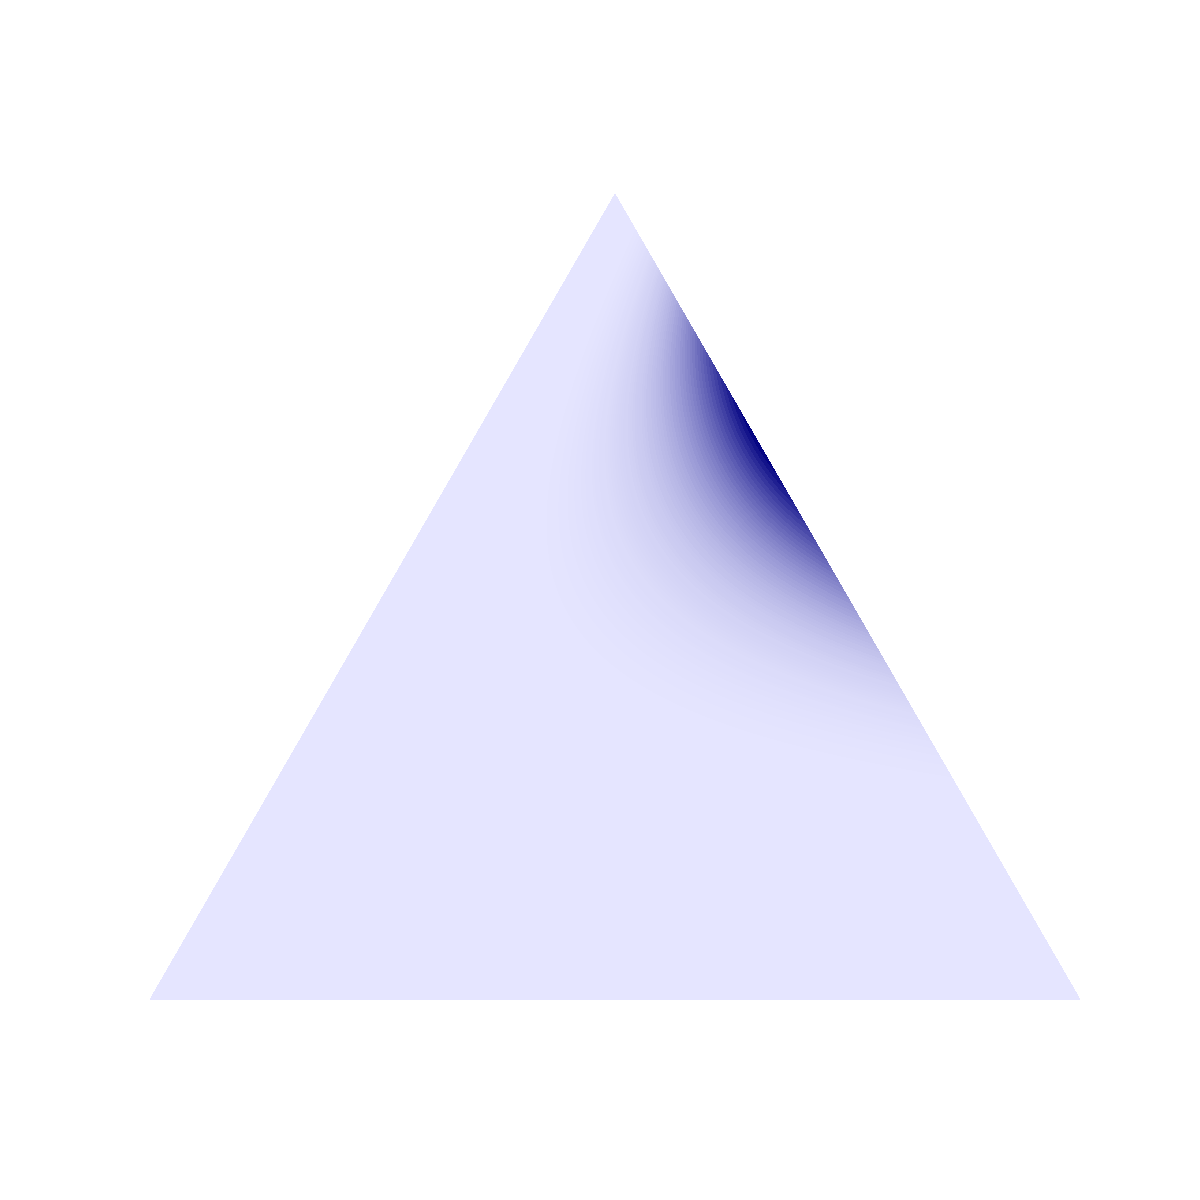
\includegraphics[width=14mm]{figs/fig1/t0.png}};  % include a picture here

 \node[triangle, draw=black, thick,inner sep=3mm](d1) at (\xb + 1.0,-2.3) {}; 
  \node[triangle, draw=black, thick,inner sep=3mm](d2) at (\xb + 2.7,-2.3) {}; 
   \node[triangle, draw=black, thick,inner sep=3mm](d3) at (\xb+4.4,-2.3) {};  
% TRIANGLE PICTURES HERE
 \node (t11) at (\xb + 1.0,-2.3+0.2) {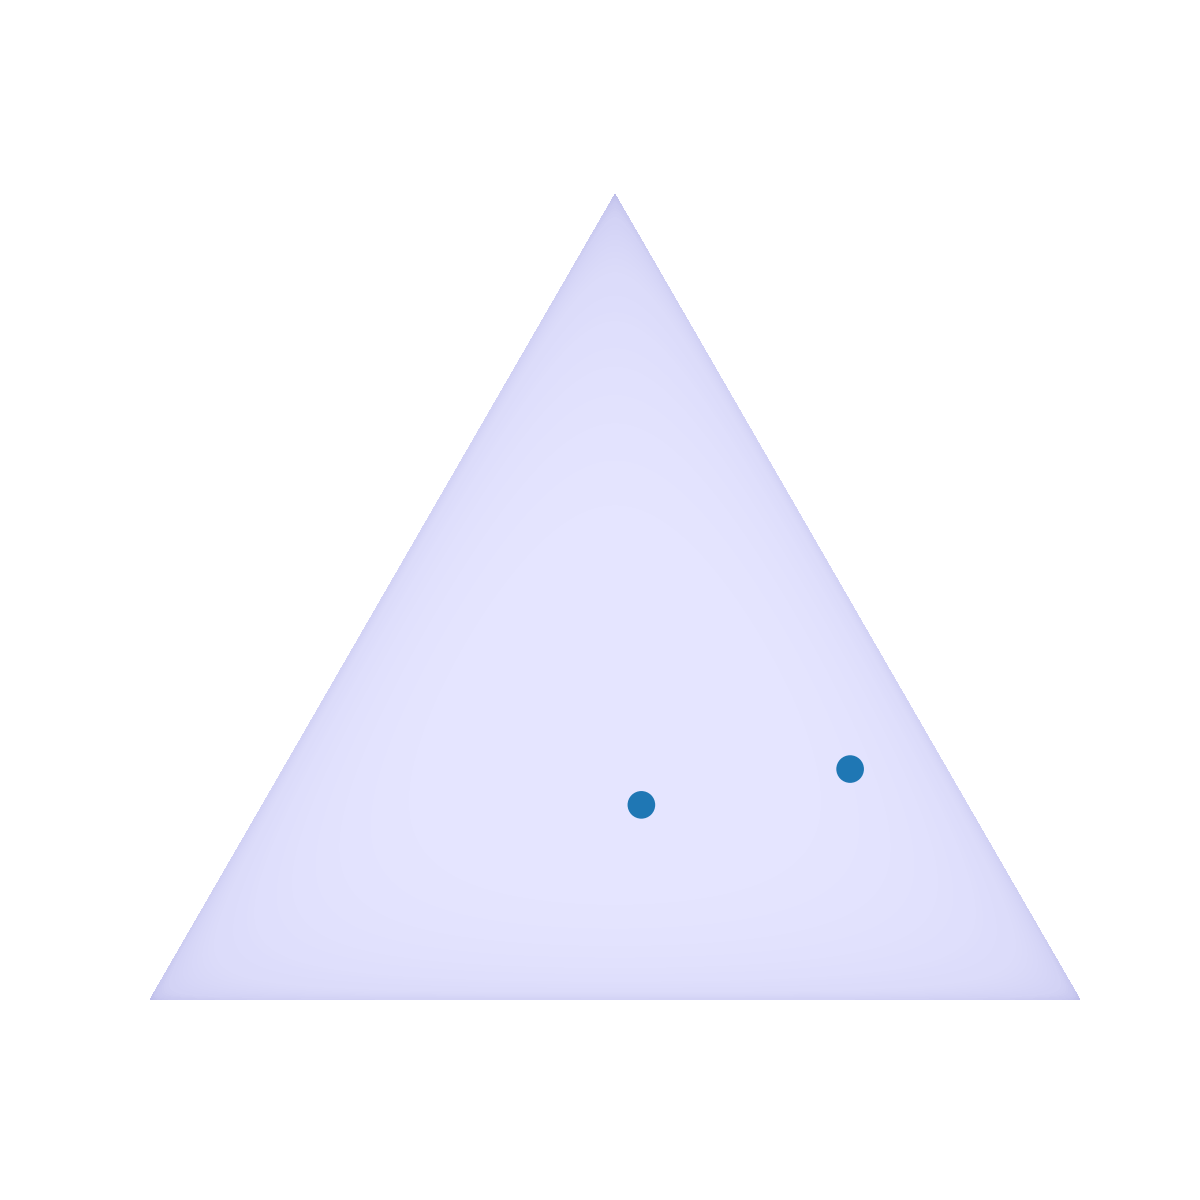
\includegraphics[width=14mm]{figs/fig1/t11.png}};  % include a picture here
 \node (t12) at (\xb + 2.7,-2.3+0.2) {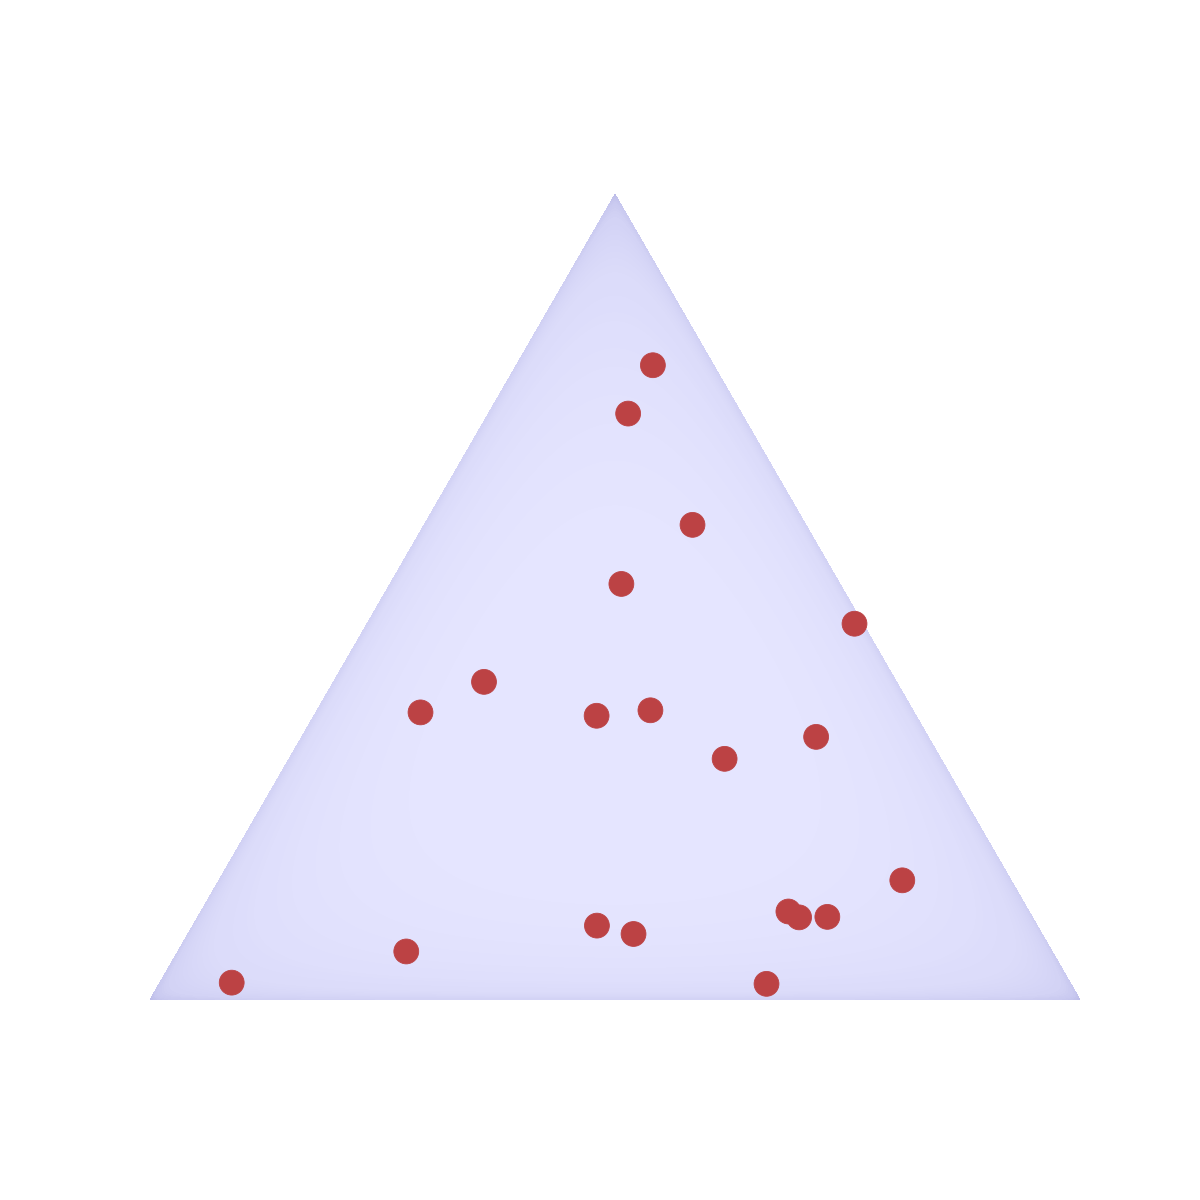
\includegraphics[width=14mm]{figs/fig1/t12.png}};  % include a picture here
 \node (t13) at (\xb + 4.4,-2.3+0.2) {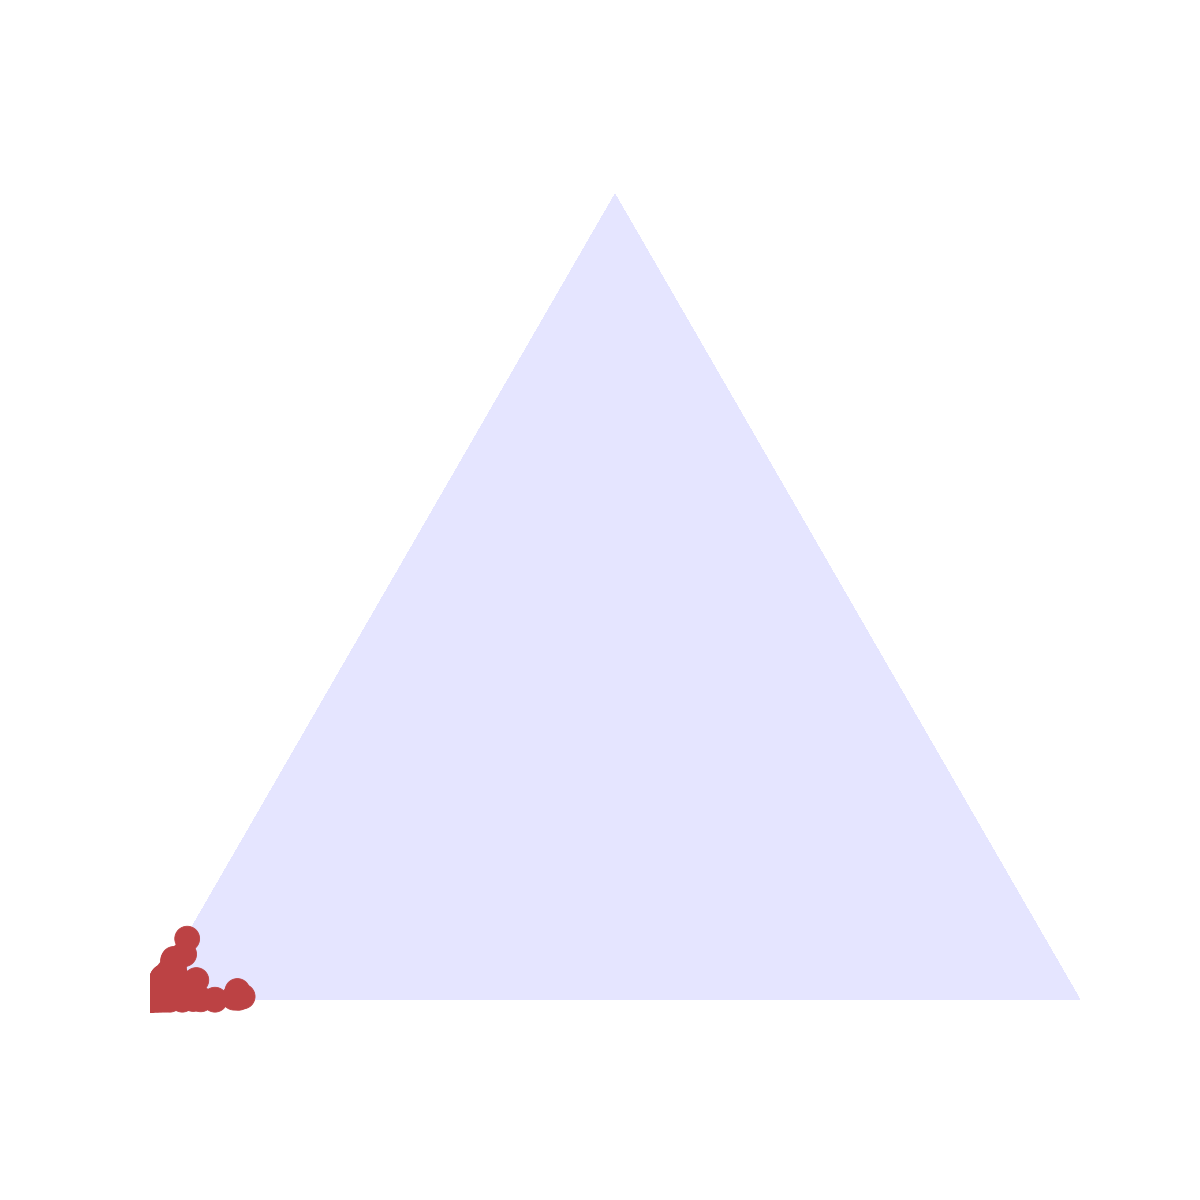
\includegraphics[width=14mm]{figs/fig1/t13.png}};  % include a picture here

  \node (dt) at (\xb + 3.5,-2.1){...};

 \node[triangle, draw=black, thick,inner sep=3mm](dp1) at (\xb + 1.0,-4.7) {}; 
  \node[triangle, draw=black, thick,inner sep=3mm](dp2) at (\xb + 2.7,-4.7) {}; 
   \node[triangle, draw=black, thick,inner sep=3mm](dp3) at (\xb + 4.4,-4.7) {};  
% TRIANGLE PICTURES HERE
 \node (t21) at (\xb + 1.0,-4.7+0.2) {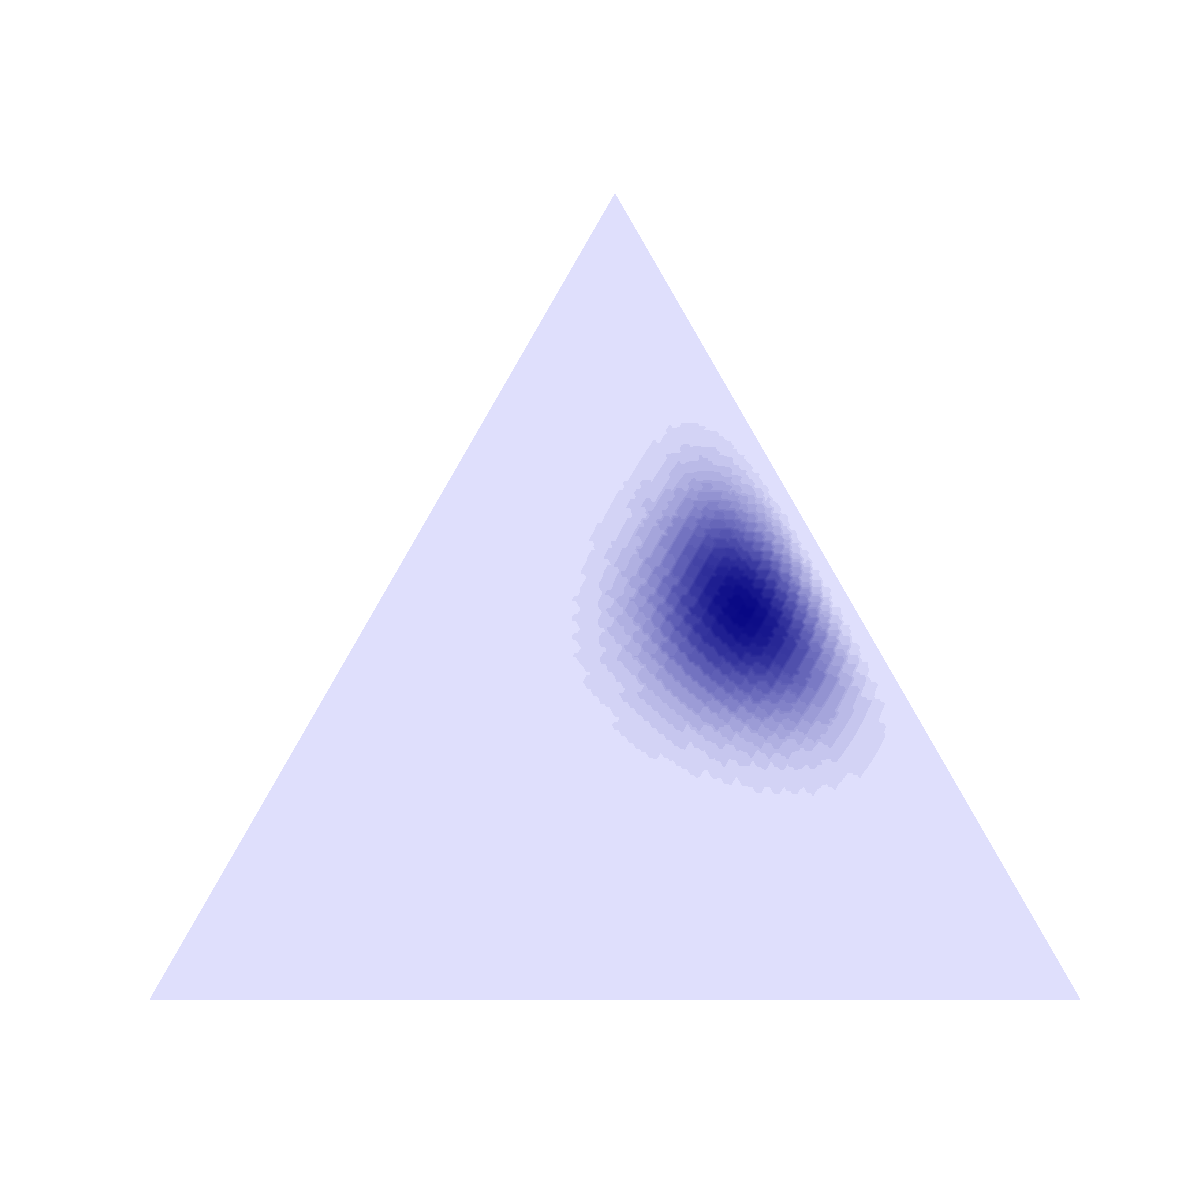
\includegraphics[width=14mm]{figs/fig1/t21.png}};  % include a picture here
 \node (t22) at (\xb + 2.7,-4.7+0.2) {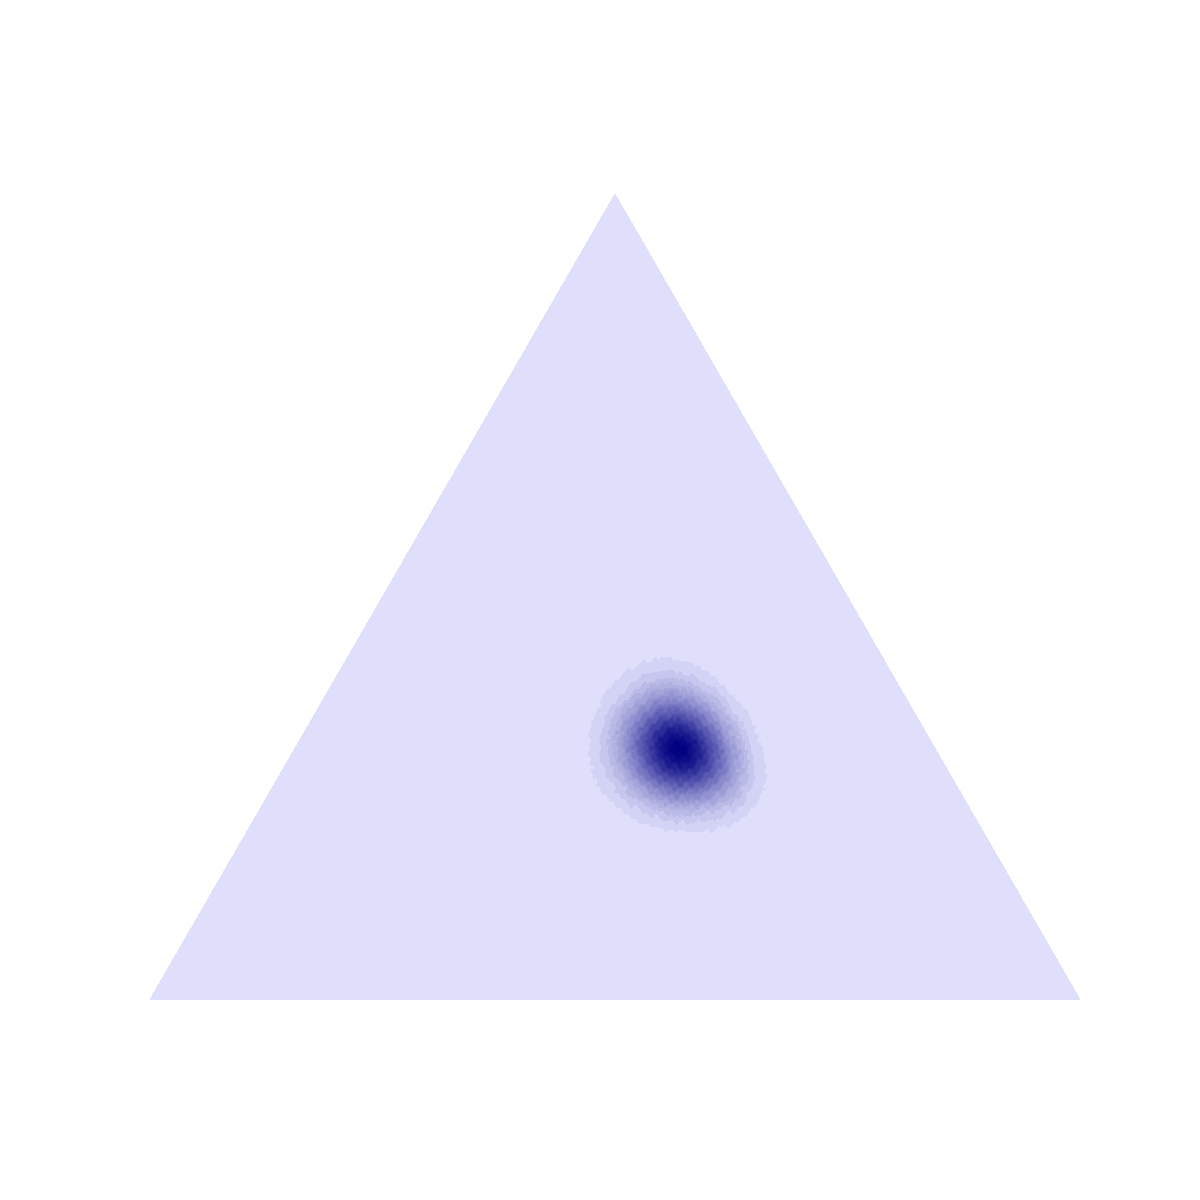
\includegraphics[width=14mm]{figs/fig1/t22.png}};  % include a picture here
 \node (t23) at (\xb + 4.4,-4.7+0.2) {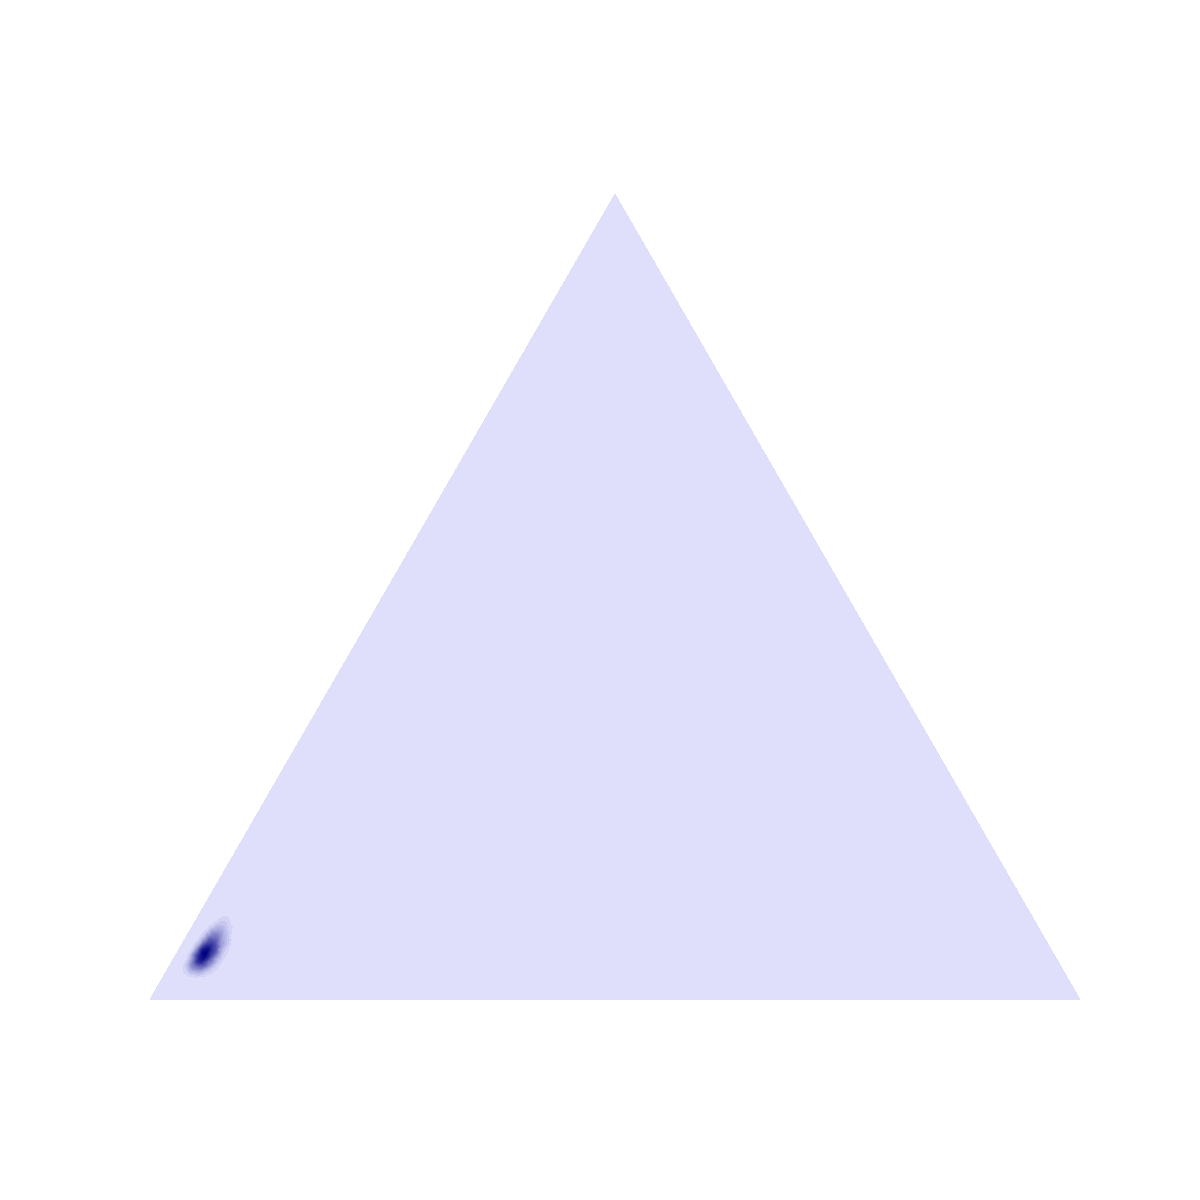
\includegraphics[width=14mm]{figs/fig1/t23.png}};  % include a picture here

  \node (dpt) at (\xb + 3.5,-4.3){...};

 \node (p1) at (\xb + 1.0,-2.8) {};
  \node (p2) at (\xb + 2.7,-2.8) {};
   \node (p3) at (\xb + 4.4,-2.8) {};
\draw[thick,dashed,->] (p1)--(dp1); 
\draw[thick,dashed,->] (p2)--(dp2); 
\draw[thick,dashed,->] (p3)--(dp3); 

\draw[thick,->] (d0.south)--(d1.north); 
\draw[thick,->] (d0.south)--(d2.north); 
\draw[thick,->] (d0.south)--(d3.north); 


% panel C
\node (C) at (\xc, 0.4) {{\bf C}};

\node (w) at (\xc+1.5,0.0) {$w \sim \mathcal{N}(0,I)$};

\node (nf1) at (\xc+1.5, -1.1)  {};
\draw[draw=black,thick] (\xc+0.5, -1.2) rectangle ++(2.2,0.2);
\draw[thick,->] (w.south)--(nf1.north);

\node (nf2) at (\xc+1.5, -2.1)  {};
\draw[draw=black,thick] (\xc+0.5, -2.2) rectangle ++(2.2,0.2);
\draw[thick,->] (nf1.south)--(nf2.north);

\node (nf3) at (\xc+1.5, -3.1)  {};
\draw[draw=black,thick] (\xc+0.5, -3.2) rectangle ++(2.2,0.2);
\draw[thick,dotted] (nf2.south)--(nf3.north);

\node (nf4) at (\xc+1.5, -4.4)  {$z \sim q_\phi(z;\eta)$};
\draw[thick,->] (nf3.south)--(nf4.north);

% now the theta of eta network.
\node (eta) at (\xc+5.6, -2.1) {$\eta$};

\node (te1) at (\xc+4.9, -2.1)  {};
\draw[draw=black,thick] (\xc+4.8, -3.2) rectangle ++(0.2,2.2);
\draw[thick,->] (eta)--(te1);

\node (te2) at (\xc+4.3, -2.1)  {};
\draw[draw=black,thick] (\xc+4.2, -3.2) rectangle ++(0.2,2.2);
\draw[thick,->] (te1)--(te2);

\node (te3) at (\xc+3.7, -2.1)  {};
\draw[draw=black,thick] (\xc+3.6, -3.2) rectangle ++(0.2,2.2);
\draw[thick,dotted] (te2)--(te3);


% connect networks
\node (nf1r) at (\xc+2.6, -1.1)  {};
\node (nf2r) at (\xc+2.6, -2.1)  {};
\node (nf3r) at (\xc+2.6, -3.1)  {};
\draw[thick,->] (te3)--(nf1r); 
\draw[thick,->] (te3)--(nf2r); 
\draw[thick,->] (te3)--(nf3r); 

\node (tpe) at (\xc+2.4, -2.5) {$\theta_{\phi} (\eta)$};
\node (phi) at (\xc+4.3, -3.5) {$\phi$};


% \xnode (x) at (-4.0,-2.0) {$x$};
% \znode (z) at (-4.0,0.0) {$z$};
% \node (a) at (-5.0,-2.0) {$\gamma$};
% \node (a0) at (-5.0,0.0) {$\alpha_0$};
%
%  \draw[thick] (x)--(z);
%  \draw[thick] (a0)--(z); 
%  \draw[thick] (a)--(x);
%  
  
%  \gmnode (X) at (0,0) {};
%  \node[align=center] at (X)        {$\sigma\left(\sum_i \!w_{ij}^0 x_{i}^0 \!+\! b_j^1\right)$};
%  \node (X1) at (-3.0,-2.0) {$x_{3}^0$};
%  \node (X2) at (-3.0,0) {$x_{2}^0$};
%  \node (X3) at (-3.0,2.0) {$x_{1}^0$};
%  \node[circle,fill=black] (X4) at (2.5,0) {};
%  \node (X5) at (4.0,-2.0) {...};
%  \node (X6) at (4.0,0.0) {...};
%  \node (X7) at (4.0,2.0) {...};
%  \node (X8) at (1,-2.5) {Neural unit};
%  
%  \draw[thick] (X)--(X1) node[pos=0.8,scale=0.2,label=right:{$w_{3j}^0$}] {};
%  \draw[thick] (X)--(X2) node[pos=0.5,scale=0.2,label=above:{$w_{2j}^0$}] {};
%  \draw[thick] (X)--(X3) node[pos=0.8,scale=0.2,label=right:{$w_{1j}^0$}] {};
%  \draw[thick] (X)--(X4) node[pos=0.5,scale=0.2,label=above:{$x_j^1$}] {};
%  \draw[thick] (X4)--(X5) ;
%  \draw[thick] (X4)--(X6);
%  \draw[thick] (X4)--(X7) node[pos=0.5,scale=0.2,label=right:{}] {};

% \node[obs]                   (x)      {$x$} ; %
%  %\node[latent, above=of T]    (theta)  {$\theta$}; %
%%\node[const, above=of x] (f) {};
%  \node[latent, above=of x]    (z)      {$z$} ; %
%  \node[const, left=of z] (a0) {$\alpha_0$};
%
%\edge {z}{x};
%\edge {a0}{z};
%

%  \plate {plate1} { (x) } {$N$}; %
 
%  % More nodes
%  \factoredge {x}  {z}     {x} ; %
% % Define nodes
%  \node[obs]                               (y) {$y$};
%  \node[latent, above=of y, xshift=-1.2cm] (w) {$\mathbf{w}$};
%  \node[latent, above=of y, xshift=1.2cm]  (x) {$\mathbf{x}$};
%  \node[latent, right=2cm of y]            (t) {$\tau$};
%
%  % Connect the nodes
%  \edge {x,w,t} {y} ; %
%
%  % Plates
%  \plate {yx} {(x)(y)} {$N$} ;
%  \plate {} {(w)(y)(yx.north west)(yx.south west)} {$M$} ;

 
 
  
\end{tikzpicture}

  \caption{Learning exponential families.  A shows the graphical model, emphasizing conditional iid sampling.  B shows Dirichlet prior (a density), conditional Dirichlet observations (some observed points in the simplex), and then the posteriors learned by an EFN.  SRB to fill in these triangles.   C shows the EFN network schematic.}
\end{figure}

 %%%%%%%%%%%%%%%%%%%%%%%%%%%%
 \subsection{Exponential families as target models}

We will focus on a fundamental problem setup in probabilistic inference, that of a latent variable $z \in \mathcal{Z}$ with prior belief $p_0(z)$, and where we observe a dataset $X = \left\{x_1,...,x_N\right\} \subset \mathcal{X}$ as conditionally independent draws given $z$.   Updating our belief with data produces the posterior $p(z | X) \propto p_0(z) \prod_{i=1}^N p(x_i | z)$.  This setup is shown as a graphical model in Figure 1A.

In rare cases these posterior distributions are tractable due to either known conjugacy or to careful historical work (often an inversion, transformation-rejection, or similar custom numerical strategy) that has made these distributions computationally indistinguishable from tractable \cite{Devroye:1986aa}.  It is intriguing then to reflect upon the success that deep networks have offered to function approximation, and ask to what extent we can automate this numerical process, widening the class of effectively tractable distributions.

If we restrict our attention to priors and likelihoods that belong to exponential families $\mathcal{P} = \left\{ \frac{h(\cdot)}{A(\eta)} \exp\left\{ \eta^\top t(\cdot) \right \} : \eta \in H \right\}$, the posterior can be also viewed as an exponential family, albeit intractable \cite{wainwright2008graphical}.  For simplicity we will hereafter suppress the base measure $h(\cdot)$.  Consider:

$$ p_0(z) = \frac{1}{A_0(\alpha)} \exp\left\{ \alpha^\top t_0(z) \right \} ~~~ , ~~~ p(x_i|z) = \frac{1}{A(z)} \exp\left\{ \nu(z)^\top t(x_i) \right \},$$

where $t(\cdot)$ is the sufficient statistic vector, and $\nu(z)$ is the natural parameter of the likelihood in natural form \cite{robert2007bayesian}.   The posterior then has the form:

$$  p(z | x_1,...,x_N)  \propto  \exp\left\{ \begin{bmatrix} \alpha \\ \sum_i t(x_i) \\ -N \end{bmatrix}^\top\begin{bmatrix} t_0(z) \\ \nu(z) \\ \log A(z) \end{bmatrix} \right\},$$

which again is an exponential family, albeit intractable.

To give a concrete example, consider the hierarchical Dirichlet -- a Dirichlet prior $z\sim Dir(\alpha)$ with conditionally iid Dirichlet draws $x_i | z \sim Dir(\beta z)$, which has been considered historically \cite{mackay1995hierarchical}, has relevance for multi-corpus topic models \cite{blei2003latent, pritchard2000inference}, and is perhaps most notable for its nonparametric extension \cite{teh2006hdp} (and has relevance for .  Figure 1B shows the prior for a given $\alpha$ (top), and three examples of datasets that could arise via this generative model (middle).  A set of basic manipulations shows the hierarchical Dirichlet posterior $p(z|X)$ to be itself an exponential family with natural parameter $\eta = \left[ \alpha -1 , \sum_i \log(x_i) , -N \right]^\top$ and sufficient statistic $t(z) = \left[ \log(z), \beta z , \log(B(\beta z)) \right]$.  The corresponding posteriors are shown in Figure 1B (bottom).  

The point is that this example, and intractable exponential families generally, form a probability model that we would like to learn.  Should we be able to learn this family (in the sense of making it tractable)




define $\mathcal{P}$.  Lay down notation.  Ref Fig 1a and Fig 1b.

bants.  Pitman-Koopman Lemma \cite[\S 3.3.3]{robert2007bayesian}  Defines an M.  


%Note briefly that one common model that this does not conveniently include is local latent variable models like LDA and logistic regression, as they define larger and larger exp fams as they go (yes they are exp fams, but not of a fixed parameterization under sampling).
%
% Note somewhere that the natural parameter space needs to be considered in general.  That is, not all $\eta$ lead to a valid distribution (standard fact, see for example \cite{wainwright2008graphical}).  In practice that's not often a problem, as the space is known for most distributions one uses, and when one composes them in a posterior scheme (for example), this is inherited (eg the normal covariance...).  So we skip that here.  But yes in general that needs to be considered.


%%%%%%%%%%%%%%%%%%%%%%%%%%%%
 \subsection{Density networks as approximating family}

Implicit probability models can be defined by any base random variable $w\sim p_0$ mapped through any measurable, parameter-indexed function family  $\mathcal{G} = \left\{g_\theta: \theta \in \Theta\right\}$; we denote the induced density on $z=g_\theta(w)$ as $q_\theta(z)$.   
Though trivial to sample from $q_\theta(z)$ for any choice of family $\mathcal{G}$, we here additionally require that we be able to explicitly calculate $q_\theta(z)$.  
This goal can be readily achieved by designing $\mathcal{G}$ to contain only bijective functions, ideally with a Jacobian form that is convenient to compute. %such that $q_\theta(z) = \frac{1}{|J_\theta(z)|} q_0\left(g_\theta^{-1}(z)\right)$ is convenient to compute.   
Designing that bijective $\mathcal{G}$ as a deep neural network family, as we do here, is a well-established idea that has recently seen many variants and applications \cite{mackay1997density, baird2005one, tabak2010density, rippel2013high, uria2013rnade, rezende2015variational, dinh2016density, papamakarios2017masked, jacobsen2018revnet}.  Specifically, let $z = g_\theta(w) = g_L \circ ... \circ g_1(w)$ for bijective vector-valued functions $g_\ell$ (where for clarity we have surpressed the dependence of each on $\theta$), and denote $J_\ell$ as the Jacobian of the function $g_\ell$.  Then we have:
%
$$q_\theta(z) = q_0\left( g_1^{-1} \circ ... \circ g_L^{-1}(z) \right) \prod_{\ell=1}^L | J_\ell^{-1} |.$$
%
The specific form of the layers $g_\ell$ can be chosen based on empirical considerations; we clarify our choice in \S3.  For the remainder (and to avoid confusion when we introduce a second network) we call this deep bijective neural architecture the \emph{density network}; this network is shown vertically oriented (flowing from $w$ down to $z$) in Figure 1C.

%Note that what norm flows  \cite{rezende2015variational} did is make it tractable and scalable and in the modern VAE style, and even that is probably overstating the case.  That makes these comparisons legitimate and apples to apples.   Gaussianization is an old idea that this is basically the inverse of \cite{chen2001gaussianization}; same idea in more depth and that argues for the normal prior in \cite{tabak2010density}.  Really the norm flow is not so special as this is a well established classic idea.    
 

 %%%%%%%%%%%%%%%%%%%%%%%%%%%%
 \subsection{Exponential family networks}

includes the network definition of Fig 1c, the objective, and the optimization algorithm.
 
This should not be confused with "Learning to learn by gradient descent by gradient descent" \cite{andrychowicz2016learning} 

Another related work is that this is somehow the dual of MEFN \cite{loaiza2017maximum}, or a generalization of the dual problem.  In the wainwright and jordan sense of forward and backward mappings.
Stuff on sampling from Gibbs distributions (max ent models), and sampling from exp fams generally, with MCMC and such.

Note that this objective can also produce approximations of the log partition, via essentially linear regression; more nuanced schemes are recommended \cite{papamakarios2015distilling}.  We don't explore that here.


 %%%%%%%%%%%%%%%%%%%%%%%%%%%%
 \subsection{Relation to variational inference}
 
 We have already covered related work; here we scrutinize EFNs in terms of VI.
 
We are interested in perhaps the most classic inference problem:

$$p(z | x) \propto p(z) \prod_{i=1}^n p(x_i | z)$$

 shown with the attached plate model (not local latents).  Supposing as is often the case that the likelihood is a member of the $s$ exp fam, we have:
 
 $$p(z | x ) \propto \exp\left\{ \left[ \sum_{i=1}^n s(x_i) \right]^\top\left[ t(z) \right] + g_0(\alpha,z) \right\}$$
 
 Important to distinguish carefully from VI.  In a sense VI does parameterize a family: given data, you get local variational parameters and that parmaterizes a density (like a regular VAE).  Inference networks are exclusively used to data to amortize with a global set of parameters a variational distribution, not a model.  Of course it is in a sense a model, but that's a bunch of normals.  The sampling mechanism is easy (Guassian).  
 
 where the natural parameters of the sampling distribution are indexed by the latent parameter on which we want to inference ($z$).  Here I've written the prior as arbitrary, and possibly not exp fam, which is fine, since this is still an exp fam in the  sense of, for a fixed $\alpha$, the function $g_0$ can just be viewed as a sufficient statistic.  Even if $\alpha$ is not fixed though, we can sample over that too to learn the whole fam (but maybe not if we want to infer it?).  Regardless, life is simpler to make sense of if we take an exp fam prior $g_0(\alpha,z) = \alpha^\top t_0(z)$, and then the desired posterior is an intractable exp fam, but still just an exp fam.
 
 Note: consider changing all $z$ to $\theta$ to remind the average reader that we're doing real bayesian inference and not just run of the mill VI with local latents in a nonlinear dimension reduction setting.  Perhaps an important reminder that most all of VAE and such are for inference of local latents, and that's a little bit too bad.  We fix that.

Another key  idea that EFNs enable is to ask if learning the $\theta(\eta)$ network leads to better VI in terms of inference networks, since it is apparently appropriately regularized and can just take suff stats.  That's testable if we have time.

In a restricted technical sense, rather close: VAE and other black box VI that uses reparameterization results in a conditional density $q_\phi( z | x)$.  If we consider $\eta$ as $x$, then sure yes the previous stuff specifies a model $\mathcal{Q}_{VAE} = \left\{q_\phi(z|x) : x \in X\right\}$.  But that's a little silly, and any way that is very often a normal family with variational parameters specified by (a deep function of) x.  Much closer is Figure 2 in Rezende and Mohamed, where like here they use a network to index the \emph{parameters} of the normalizing flow.  In that case it's a function of $x$ the observation, and as such that network is an inference network; here it's a function of $\eta$ and as such is a parameter network.  That's just nomenclature, so naturally the next question is do they differ at some other level.  Yes, distinctly.  The other term implied in a VI (or norm flow VAE style as they use) is the expected log joint $E_{q_{\phi(x)}}  \left( \log p_\theta(x,z)\right)$.  Now sure that's a loss function on $x,z$, so then when we look at that same term in EFN we see   $E_{q_{\phi(\eta)}}  \left( \eta^\top t(z) \right)$, which sure also looks like a loss function on $\eta,z$.  And yes, they are both unnormalized (in the sense that VI is an ELBO / joint $p(x,z)$ and EFN lacks the normalizer because it's constant, so we're not getting a KL estimate).  A picky difference is that the exp family doesn't really correspond to a proper unnormalized log joint (though I suppose it could), as there is not a prior on $\eta$ in the objective (but is that just ignoring $p(\eta)$ in our sampling scheme?). But yes if we want to be reductionist and pedantic [use nicer words] in general we could see this as a specific case where $x=\eta$ and thus we are learning a family just as in the inference case.  Or rather, we are putting the data in as sufficient stat (computation of natural parameters), but that's nonobvious.  And for example we are giving in the bayesian logistic regression example full datasets for inference instead of single data points.  To make this as close as possible, we write $p(\eta | z)  = \frac{1}{A(t(z))} \exp\left\{ \eta^\top t(z)\right\}$.  That's the "likelihood" of an EFN in some wonky sense.  So this reveals the mechanical differences: first, $t(z)$ is not a deep generative model with parameters $\theta$, but rather it is a fixed set of sufficient statistics that define the exp fam.  Next, there is no clear prior $p(z)$, which is critical to understanding how VI behaves (see Hoffman and Johnson ELBO surgery paper, also Duvenaud's https://arxiv.org/pdf/1801.03558.pdf).  So yes there is a hand wavy sense in which EFN is a specific case of norm flow, but of course it is.  And anyway norm flow is a specific case of a DNN architecture or Helmholtz machine or deep density network (Ripple and Adams).  This is just rambling but good to have all perspective here.  Ok so what to do?  First, then we need to produce really compelling results focusing on when learning an exp fam is key.  Second we need some very tight language to draw this distinction without seeming a small tweak on normalizing flows.  One way to do this is the restricted model class argument, a la Fig 7.2 in Hastie and Tibshirani.  Another is to actually produce a conditional exp fam, as in something indexed on both $x$ and $\eta$.  Third, possible novelties in norm flows, like triple spinners or other better choices than planar flows (yuck).

  Another point is that it's unknown if posterior contraction can be well modeled.  As in, we know that most VI NF type things are conditioned on a single data point, so the posterior variance can tend to be rather homogenous.  One more contribution is to offer that contraction study; as we get more data points we will get more posterior contraction, so this tests the ability of this model to learn that.
  
  Key distinctions:
  \begin{itemize}
  \item narrow mechanical sense this is VI with an observation of the natural parameters, namely the sample exp fam over all data.  but that's pedantic.
  \item no generative model in the usual sense: yes, we can consider a prior and then some observation model as the genrative model, but in any event it's not a neural net.
  \item we lack a finite data set $X$, so the objective is technically different.  We stipulate a distribution and then this is expectation over that model space, a KL or a KL to the broader joint with $\eta$.  This is concretely different, as we typically use a fixed size dataset $X$ so we can calculate the ELBO over the 
  \end{itemize}
  
Latest key distinctions:
\begin{itemize}
\item prior is in parameter network, unlike essentially all others, even if you take a narrow view that $\sum_i t(x_i)$ is a single data point.  Prior has been recognized for mattering in the ELBO, though this sentence is a dubious distinction \cite{hoffman2016elbo,cremer2018inference} (dubious need for these refs)
\item data is given via an assumption of sufficiency, namely in natural form \cite{robert2007bayesian}, not in $x$ form.  Of course this is sensible as in some settings we don't know the natural form of the generative model, but that's a key difference with SVI; plenty of those models are not deep nets (and shouldn't be, if there is an intent of statistical inference rather than nonlinear dimensionality reduction / autoencoding ) and there we \emph{do} know the natural parameters.
\end{itemize}

 
 More generally there has been a lot of attention to making these more flexible in structured variatonal inference.  Any generalization of this is also dandy though, so could use a mean field approach (standard) or any of the things that go beyond mean field, either classically \cite{saul1996exploiting, barber1999tractable}; this is called structured variational inference or newer stuff  \cite{hoffman2015stochastic} \cite{tran2015copula}, to name but a few.

 


  
%%%%%%%%%%%%%%%%%%%%%%%%%%  
\section{Results}

Introductory remarks and then comments about architectural particulars, including planar flow networks of \cite{rezende2015variational}. Note Number of panar flows is always D (intrinsic dimensionality of flows), units per layer ramping is always the same function of D.  The number of layers in the theta network is always a function of D - will probably just always use 8 layers.
Remember 

NF1: do full norm flow ``variational inference'' (explore all of $\phi$ space with the full flow network model $\mathcal{Q}$), which is to say $\arg\min_\phi KL(q_\phi || p)$.  

EFN1:  be literal to Figure 1C, give the sufficient statistics of that K=1 dataset, and learn an EFN from scratch.  This alternative is important because it is the most specific (but kind of annoying, hence alternative 1) interpretation of norm flow VI paper.  

\subsection{Tractable exponential families}

 \begin{figure}
  \centering
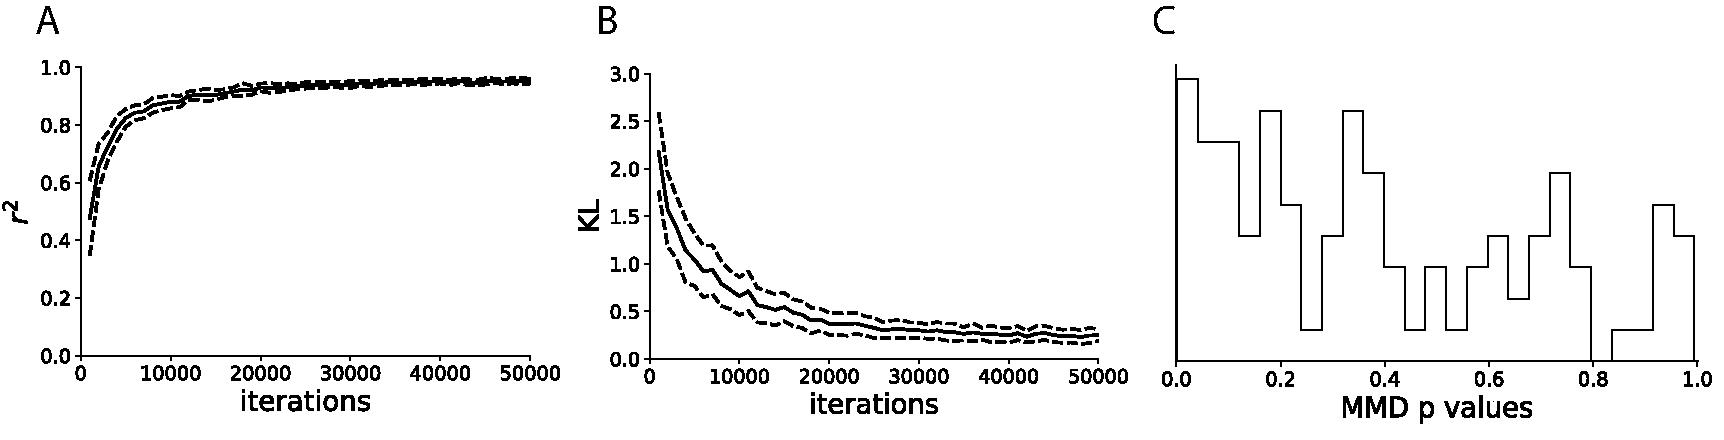
\includegraphics[scale=0.46]{figs/fig2/fig2.pdf}
  \caption{25-dimensional Dirichlet exopnential family network.  A.) Distribution of $r^2$ between the sufficient statistics and log-probability across choices of $\eta$ throughout optimization.  B.) Distribution of KL divergence across choices of $\eta$ throughout optimization.  C.) Distribution of maximum mean discrepancy p-values between EFN samples and ground truth after optimization \cite{gretton2012kernel}.}
\end{figure}

 \begin{figure}
  \centering
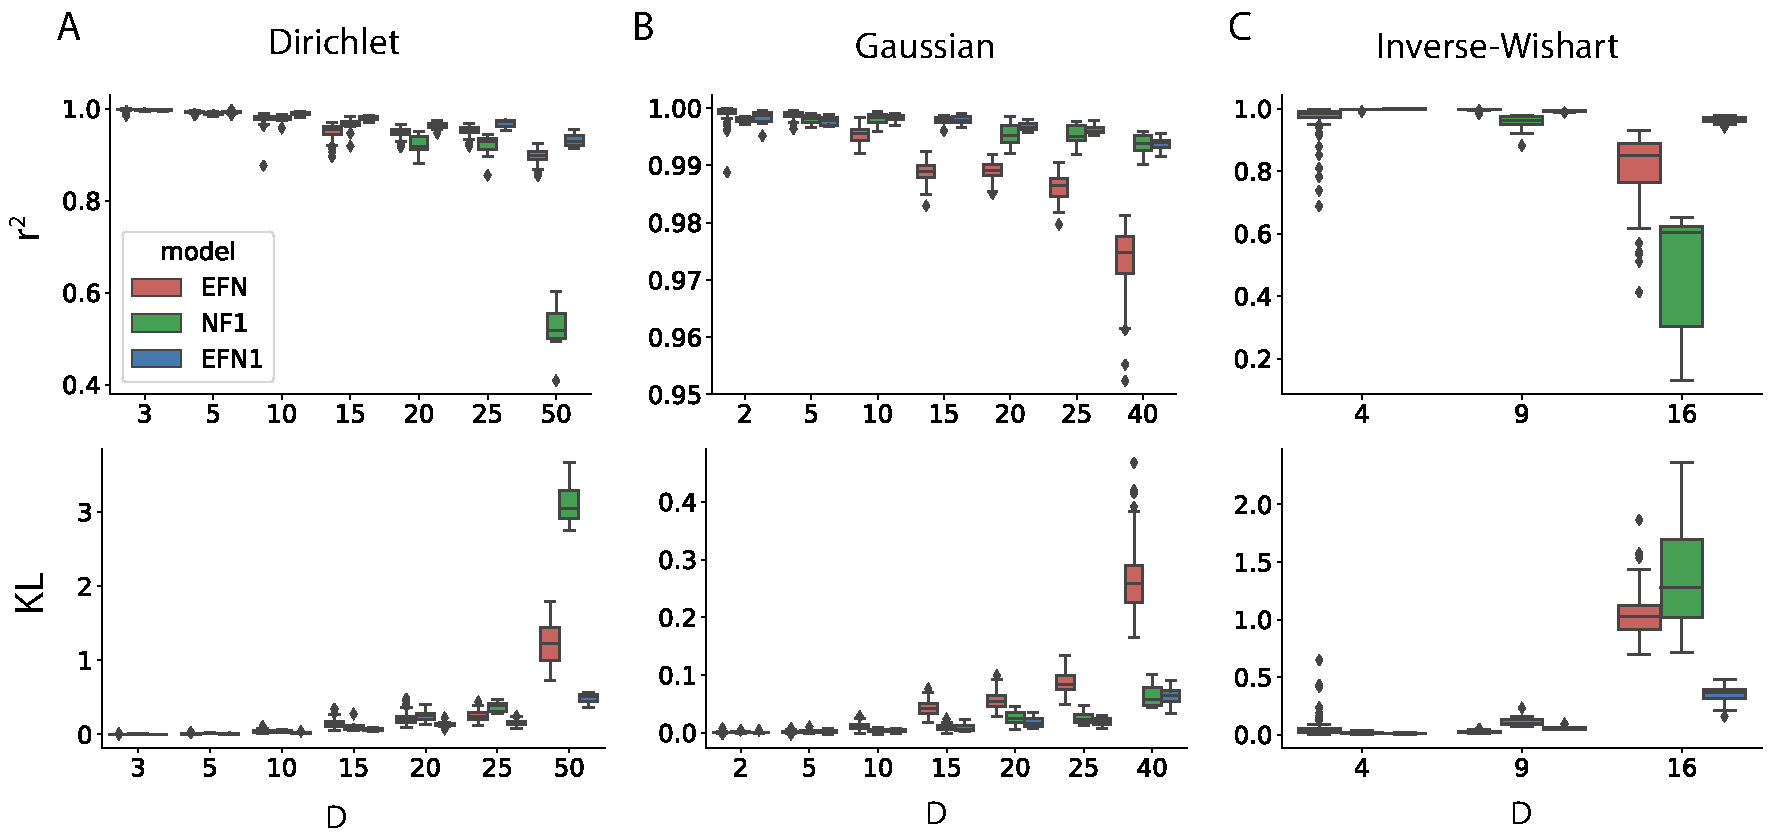
\includegraphics[scale=0.46]{figs/fig3/fig3.pdf}
  \caption{Scaling exponential family networks.  A.) Dirichlet.  B.) Gaussian  C.) Inverse-Wishart}
\end{figure}

\subsection{Intractable exponential families}


\paragraph{Hierarchical Dirichlets}

Hierarchical dirichlets are useful and have some history; most notable is with the  Hierarchical Dirichlet Process \cite{teh2006hdp}, but historically this was done in the finite case also \cite{mackay1995hierarchical}.  Here is some math.    Note that this matters for multi-corpus LDA generally as well \cite{blei2003latent, pritchard2000inference}.


\paragraph{Truncated- and log-normal Poisson}

used a lot \cite{gao2016linear}\cite{adams2009tractable}\cite{cunningham2008fast,cunningham2008inferring}

Figure 4: \\
EFN in intractable exp fams (connecting to above, but with hard distribs and the ELBO) \\
Panel A: Dir-Dir ELBO by dimensionality for NF1 and EFN and EFN1\\
Panel B: Dir-Dir ELBO by dimensionality for EFN1 vs EFN1a vs 1b vs 1c vs NF1 (with $N=1$ data point)\\


\subsection{Neural spike train analysis}

Figure 5: \\
Panel A TNP picture example of prior and posterior with a few samples, just for feel good  \\
PANEL B: ELBO on held out data as a function of $R$, for a middle choice of training dataset size $N$ and $D$. \\ 
PANEL C: ELBO on held out data as a function of $N$, for a middle choice of number of samples in the posterior $R$. \\


PANEL D (optional): (ELBO EFN - ELBO NF1) as a surface plot as a function of $R,N$.  That is, positive places is where EFN outperforms, negative NF1. \\  
The key point with these is that, while you have the \emph{same exact} flow network architecture, now you have to optimize over $\phi$ with a limited single dataset.  Learning a restricted model space is good for the bias-variance tradeoff!  Do this many times so that variance will become clear.  


---other thoughts---
Real data analysis and posterior inference.  {\bf Key real data result on TNP}.  \\
Get some data from CRCNS that has many spike trains $x_i$ for $i=1,...,N$ (ask Gabriel, as he has done some poking around recently; or look at some of the above TNP/LNP refs). \\
Those spike trains should be conditionally independent draws from the same underlying intensity function $z$.  (for example, trials under the same stimulus)\\
Bin the length of time $T$ into $\approx 20-30$ equally spaced time bins.  Thus $z$ is now a vector in $\mathbb{R}^20$. \\
Now each spike train $x_i$ is a conditionally independent Poisson vector observation, with rate vector $z$.\\
Learn the 20 dimensional TNP exp fam, without any regard to this dataset $X$. \\
No: Panel No: TNP ELBO by dimensionality for NF1 and EFN and EFN1 \\
Panel A TNP picture example of prior and posterior with a few samples, just for feel good  \\

{\bf Now we want to learn the posterior $p(z | \textrm{ some fixed number $R$ of data points})$}.  \\
To do this for an EFN, just plug in those $R$ points $x_{i_1},...,x_{i_R}$ and the prior as a natural parameter, and job done. \\
To do this for an NF1, train a VI model by taking the log joint with $R$ data points, then go through and resample $R$ points every time from your training dataset with $N$ data points. \\
{\bf PANEL A: ELBO on held out data as a function of $R$, for a middle choice of training dataset size $N$.} \\ 
{\bf PANEL B: ELBO on held out data as a function of $N$, for a middle choice of number of samples in the posterior $R$.} \\
{\bf PANEL C: (ELBO EFN - ELBO NF1) as a surface plot as a function of $R,N$.  That is, positive places is where EFN outperforms, negative NF1.} \\  
The key point with these is that, while you have the \emph{same exact} flow network architecture, now you have to optimize over $\phi$ with a limited single dataset.  Learning a restricted model space is good for the bias-variance tradeoff!  Do this many times so that variance will become clear.  
{\bf Panel C v2: Possibly want to explicitly plot variance of EFN and NF1 to focus on the variance tradeoff}\\
{\bf Panel C v3: change time bin granularity from 10 to 50 to show how this story changes in $D$.  My thought is that all will be exhausted by dimensionality sweeps by this point, so no.}\\
 also Notice one pain here is that these panels requires training a new EFN1 at every choice of $N$ and $R$ (but only one EFN).  Sorry. \\


We hope and expect this will show that when the dataset gets small, this "traditional VI" will get arbitrarily bad (can't learn a network); eventually, there will be so much data that the VI will match or outperform the EFN... outperform because VI can focus specifically on this distribution rather than over the whole family, so the EFN has less effective data for this $\eta$ (but not because it has a broader range of models, since we believe the EFN contains the closest member).  Performance metric should be ELBO on some held out data or something like that (it's a posterior, so log likelihood doesn't really make sense).  Test data anyway.   Check VI papers for usual metrics.  A key point to make here is that one great virtue of EFNs is is learning a restricted model, which should demonstrate the usual bias-variance tradeoff (see for example Hastie and Tibshirani book, Fig 7.2). Or Figure 4 is bias-variance and some sample posteriors in 2-d (showing how nicely it works), and then Fig 5 is the above performance, with both train and test.   

This will be for one real example $X$.  As such, to get error bars, just take a big dataset and randomly subsample the test set.  Then the posterior performance is really for that very dataset, so the sem is coherent and the right thing to calculate/show.  Important to clarify that doing so \emph{does not} test how well this does across the entire exp fam, but just this one posterior.  ((To test that, we would do it in simulation: generate \emph{many datasets $X$}, then do the above for every one of them.  Same computation for EFN (since its just plugging in a dataset), but VI alternatives 1 and 2 now need to be rerun for every dataset.  And it's still simulated data, not really offering something fundamentally more than Fig 3 (well ok it's an intractable model, but I'm not sure that offers so much)...let's skip that altogether)).



\section{Conclusion}

Snappy closing remarks!

%%%%%%%%%%%%%%%%%%%%%%%%%%
%\subsubsection*{Acknowledgments}
%
%Peter Orbanz.  Funding.


\clearpage
%%%%%%%%%%%%%%%%%%%%%%%%%%
%\section*{References}

\bibliographystyle{unsrt}
\bibliography{BittnerNIPS2018}
%%%%%%%%%%%%%%%%%%%%%%%%%%




%
%%%%%%%%%%%%%%%%%%%%%%%%%%%
%\clearpage
%
%\section{Appendix}
%Exponential form of posterior for Dirichlet-Dirichlet \\
%\begin{math}
%\pmb{z} \sim Dir( \pmb{\alpha}_0) \\
%\pmb{x}_i \sim Dir( \beta \pmb{z}) \\
%p(\pmb{z}) \propto \exp{(\pmb{\alpha}_0^T \log(\pmb{z}) - \sum_{d=1}^D \log(z_d)) } \\
%p(\pmb{x}_i \mid \pmb{z}) \propto \exp{(\beta \pmb{z}^T \log(\pmb{x}_i) - \sum_{d=1}^D \log(x_{i,d}) - (\sum_{d=1}^{D} \log (\Gamma (\beta z_{d})) - \log (\Gamma (\beta \sum_{d=1}^D z_{d}))))} \\
%p(X \mid \pmb{z}) \propto \exp{(\beta \pmb{z}^T \left[\sum_{i=1}^N \log(\pmb{x}_i) \right] - \sum_{i,d=1}^{N,D} \log(x_{i,d}) - N(\sum_{d=1}^{D} \log (\Gamma (\beta z_{d})) - \log (\Gamma (\beta \sum_{d=1}^D z_{d}))))} \\ 
%\end{math}
%
%\begin{math}
%p(\pmb{z} \mid X) \propto p(\pmb{z}) p(X \mid \pmb{z}) \\
%\propto \exp{(\pmb{\alpha}_0^T \log(\pmb{z}) - \sum_{d=1}^D \log(z_d))} \\
%\exp{(\beta \pmb{z}^T \left[\sum_{i=1}^N \log(\pmb{x}_i) \right] - \sum_{i,d=1}^{N,D} \log(x_{i,d}) - N(\sum_{d=1}^{D} \log (\Gamma (\beta z_{d})) - \log (\Gamma (\beta \sum_{d=1}^D z_{d}))))}
%\end{math}
%
%We don't care about the term that just has $x$ in it.
%
%\begin{math}
%p(\pmb{z} \mid X) \propto \exp{(\pmb{\alpha}_0^T \log(\pmb{z}) + \beta  \left[\sum_{i=1}^N \log(\pmb{x}_i) \right]^T \pmb{z} - \sum_{d=1}^D \log(z_d) - N(\sum_{d=1}^{D} \log (\Gamma (\beta z_{d})) - \log (\Gamma (\beta \sum_{d=1}^D z_{d}))))} \\
%p(\pmb{z} \mid X) \propto \exp{(\begin{pmatrix} \pmb{\alpha}_0 - 1 \\  \sum_{i=1}^N \log(\pmb{x}_i)  \\ -N \\ -N \end{pmatrix}^T \begin{pmatrix} \log(\pmb{z}) \\ \beta \pmb{z} \\ \log (\Gamma( \beta \pmb{z})) \\ \log (\Gamma (\beta \sum_{d=1}^D z_{d}))) \end{pmatrix})}
%\end{math}
%
%This seems right to me.  I moved $\beta$ for the second element of the natural parameters to be over with his other $\beta$-friends in the sufficient statistics.
%
%Here's a more cleaned up version:
%
%$$
%p(\pmb{z} \mid X) \propto \exp\left\{\begin{bmatrix} \pmb{\alpha}_0 - \pmb{1} \\  \sum_{i=1}^N \log(\pmb{x}_i)  \\ -N \pmb{1} \\ -N \end{bmatrix}^\top \begin{bmatrix} \log(\pmb{z}) \\ \beta \pmb{z} \\ \log (\Gamma( \beta \pmb{z})) \\ \log (\Gamma (\beta \pmb{1}^\top \pmb{z}))\end{bmatrix} \right\}  ~~\triangleq~~ \exp\left\{ \pmb{\eta}^\top t(\pmb{z}) \right\}
%$$
%
%or just using the Beta function:
%
%$$
%p(\pmb{z} \mid X) \propto \exp\left\{\begin{bmatrix} \pmb{\alpha}_0 - \pmb{1} \\  \sum_{i=1}^N \log(\pmb{x}_i)  \\ -N  \end{bmatrix}^\top \begin{bmatrix} \log(\pmb{z}) \\ \beta \pmb{z} \\ \log (B( \beta \pmb{z})) \end{bmatrix} \right\}  ~~\triangleq~~ \exp\left\{ \pmb{\eta}^\top t(\pmb{z}) \right\}
%$$
%
%
%%or not bolded \\
%%
%%$$
%%p(z \mid X) \propto \exp\left\{\begin{bmatrix} \alpha_0 - 1 \\  \sum_{i=1}^N \log(x_i)  \\ -N \\ -N\end{bmatrix}^\top \begin{bmatrix} \log(z) \\ \beta z \\ \log (\Gamma( \beta z)) \\ \log (\Gamma (\beta \sum_{d=1}^D z_{d})) \end{bmatrix} \right\}  ~~\triangleq~~ \exp\left\{ {\eta}^\top t({z}) \right\}
%%$$
%
%  
%\clearpage


\end{document}



%%%%%%%%%%%RESULTS WE WANT TO GET TO EVEN IF NOT RIGHT NOW%%%%%%%%%%%


Fig 5.  Heaps of examples with conditional iid exp fams.  Math details of that pending.  Some cool examples:
\begin{itemize}
\item Censored data.  normal prior, censored normal observations, what is posterior distribution on mean?  Lots of work in that.
\item Truncated data.  truncated mvn prior, with some observations thereafter, what is posterior? (Does this work?...)
\item Poisson/Bern "process" data.  Phony process like in neuro, normal prior on log intensity (ooh maybe that's not an exp fam prior), then a "spike train" of bern or poisson count observations
\item multivariate t with inverse wishart prior or something like that.  That's neat but doesn't have great "oh yeah people do care about that problem" recognition.  Seems contrived.
\item check MKB book for other cool MV distributions. (Marshall-Olkin)... seems contrived.
\item Elliptically contoured prior with some conditionally iid exp fam observations.  People in ML like elliptical distributions.
\item von Mises-Fisher distribution, eg http://www.jmlr.org/papers/volume6/banerjee05a/banerjee05a.pdf or https://arxiv.org/pdf/1605.00316.pdf, but again not clustering (see below), since it's a local latent variable problem then.s	
\item Note: a whole heap of models don't quite fit comfortably here.
\begin{itemize}
\item Bayesian Logistic Regression.  This is an intractable exp fam in the desired sense, but the natural parameter (when parameterized) depends on $x_i$.  Thus, it grows with every datapoint, or put differently it's a diff exp fam for every dataset.  No bueno.  This is then true of GLMs, so those are out too.
\item Latent Dirichlet Allocation.  Local variational parameters mean that the exp fam grows with datasize.  That means that the posterior is already too big for uninteresting sizes of LDA.  This is then true of hierarchical models with local latent variables in general.   
\end{itemize}

\end{itemize}



Fig 6. The Killer real data.  Perhaps Gibbs or Markov Random Field.  Learn it, then pick some $\eta$, then show samples from it.  Can this look interesting?  Some thoughts...
 
 Criteria:
 \begin{itemize}
\item Needs to be an exp fam.
\item Needs to be a forward exp fam.  As in, not fit to data, because we don't have $\mu$ parameters, we have $\eta$ parameters.
\item ``real data" is a misnomer, since we are not doing VI or similar.  Really we want an exp fam that is real and somehow useful in its own right, and that people want to sample from.
\item Reminder: we will \emph{always} be comparing to "well normally you can do this with learning a \emph{single} distribution in the $\min KL(q||p)$ sense.  That's fine.  The point is we can learn the whole family, then choose and sample, vs just one by one.
\item something hard to sample will be key, since the "toy" results will have used things we already "know" how to sample, like NIW or Dirichlet.
 \end{itemize} 

Ideas: 
\begin{itemize}
\item Fancy Exp Fam like Marshall-Olkin.  Yeah but who really cares about this esoteric distribution?  It doesn't look cool visually either.
\item Ising models: classic, bw images, but gross NP-Hard Cooper 1990.
\item Potts model: great because failure of MCMC (Gibbs sampling) here is at least locally well known from Geman and Geman 1984 through Sudderth correcting this (see Gibbs sampler slides from Advanced ML, Peter's part).  But that is kind of a failure example, not an interesting one (MRFs are smoothness prior, not segmentation prior).	Also both Potts and Ising are NP-hard Cooper 1990 The Computational Complexity of
Probabilistic Inference Using Bayesian
Belief Networks 
\item Markov Random Fields / Gibbs Random Fields (same, by Hammersley Clifford theorem).  Yes this is cool: image distributions, texture distributions.  Can show wild diff sets of textures, none of which require any sampling or any such thing.  Can we make this super intractable from an MCMC perspective?  Need to read on how sampling is done there.  Erik Sudderth and his phd thesis are likely good resources.
\item Gatys and Simoncelli texture stuff (see for example MEFN paper for refs); those are interesting distributions on textures, or specified moments.  Can then just sample from this family.
\end{itemize}  


\begin{table}
  \caption{Sample table title}
  \label{sample-table}
  \centering
  \begin{tabular}{lll}
    \toprule
    \multicolumn{2}{c}{Part}                   \\
    \cmidrule(r){1-2}
    Name     & Description     & Size ($\mu$m) \\
    \midrule
    Dendrite & Input terminal  & $\sim$100     \\
    Axon     & Output terminal & $\sim$10      \\
    Soma     & Cell body       & up to $10^6$  \\
    \bottomrule
  \end{tabular}
\end{table}


\begin{verbatim}
   \usepackage[pdftex]{graphicx} ...
   \includegraphics[width=0.8\linewidth]{myfile.pdf}
\end{verbatim}





